\documentclass[fr]{../../../../../../eplexam}
\usepackage{../../../../../../eplunits}
\usepackage{array}

\hypertitle{Mécanique des Solides Déformables}{6}{MECA}{1100}{2018}{Juin}{Mineure}
{Martin Braquet \and Michel-Antoine Fouarge}
{Issam Doghri}

\section{Théorie}

\begin{enumerate}
 \item 
    On considère une poutre droite de longueur $L$ et d'axe horizontal ($x$), encastrée en ($x=0$) et simplement appuyée en ($x=L$). La poutre est soumise à deux forces verticales $F\,\hat{\mathrm{e}}_y$ en ($x=L/3$) et en ($x=2L/3$). On souhaite calculer le déplacement vertical en ($x=L/3$) par deux théorèmes: (1) Maxwell-Betti, (2) Castigliano. Pour chacun de ces théorèmes, expliquer et illustrer graphiquement la méthode de résolution, mais sans effectuer les calculs.
 \item 
    On considère la vibration libre d'un système à un DDL: masse, ressort, amortisseur. Expliquer les 3 cas suivants: (a) amortissement critique, (b) système sous-amorti, (c) système sur-amorti. On ne demande pas d'effectuer tous les calculs, mais uniquement ceux qui permettent d'expliquer les 3 cas.
\end{enumerate}

\begin{solution}

\subsection{Maxwell-Betti}

Nous cherchons la solution (en déplacement), notée (1).\\
Pour la trouver, supposons une autre configuration, plus simple, à géométrie et matériau équivalent, dont nous pouvons trouver la solution. Nous noterons cette solution en déplacement (2). \\
Après calcul de W, le  travail du chargement compliqué (le chargement de notre problème) dans (2), il reste à déterminer (1), en sachant, par le théorème de Maxwell-Betti, que le travail du chargement simple dans ce champ (1) vaut W.

\subsection{Castigliano}

\begin{tabular}{m{7.5 cm}m{5 cm}}

Pour trouver le déplacement en $\frac{L}{3}$, posons une charge fictive Q, appliquée en A, selon la direction du déplacement ($\hat{e}_y$, car HPP). Calculons les moments (en fonction de Q) dans la structure. Par le théorème de Castigliano, 
$$\frac{\partial W}{\partial Q} = v(L/3),$$
le déplacement vertical en $L/3$. Il faut simplement imposer que $Q = -F$, et avoir le déplacement relatif à notre chargement. & 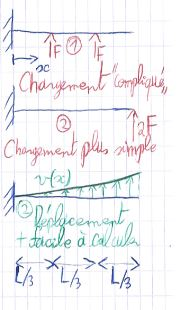
\includegraphics[scale = 1]{Castigliano.jpg}

\end{tabular}

\subsection{Vibration}

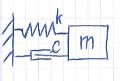
\includegraphics[scale = 1]{Vibrations.JPG}

\textbf{1. Lorsque $c = c_c$}

Qu'est-ce que $c_c$ ? L'EDO qui régit le problème de vibration est 

$$m\ddot{u} + cu' + ku = 0.$$

Son discriminant $\Delta = c^2 - 4km = 0$ (cas critique : $\Delta = 0$). Cela signifie que $c^3 = 4km \Rightarrow c = c_c = 2 \sqrt{km}$.

Après développement, la solution est une exponentielle décroissante : notre système s'amortit, mais pas de réponse harmonique ; elle ne fait pas intervenir de sinusoïde...

\textbf{2. Amortissement sous-critique : lorsque $c \leq c_c$}

La solution de l'EDO après développement sera une combinaison linéaire de sinusoïdes : il fallait développer les deux racines complexes !

\textbf{3. Amortissement sur-critique : lorsque $c \geq c_c$}

La solution de l'EDO après développement sera une combinaison d'exponentielles croissantes : il fallait développer les deux racines réelles !

\end{solution}


\section{}

On se propose d'étudier une poutre de longueur $L$ encastrée en A, simplement appuyée en B (déplacement vertical nul) et soumise à une force concentrée $F$ située à une distance $\xi$ de l'encastrement (voir figure \ref{poutre}).

\begin{figure}[!ht]
 \centering
 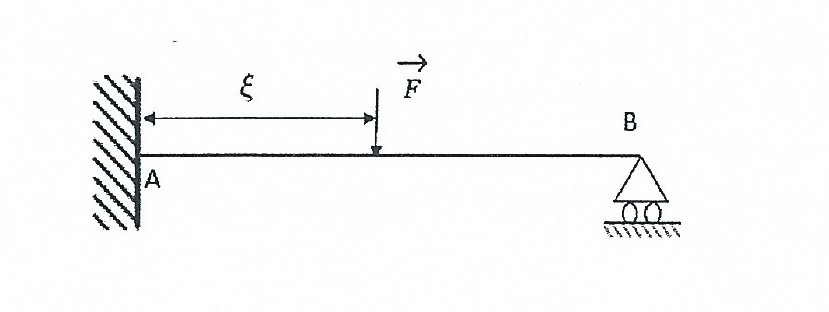
\includegraphics[width=0.7\textwidth]{Enonceun}
 \caption{}
 \label{poutre}
\end{figure}

\subsection{Partie 1}

\begin{enumerate}
 \item Calculer les réactions aux appuis A et B en choisissant la réaction au point B comme inconnue hyperstatique (on utilise Castigliano et on ne garde que l'énergie de déformation due au moment fléchissant).
 \item Dessiner les diagrammes des efforts internes en indiquant les signes et les valeurs remarquables.
 \item Calculer la flèche $v(x)$ en tout point de la fibre moyenne.
 \item Au lieu de la force concentrée, on considère maintenant une charge $q\,\SI{}{[N/m]}$ répartie uniformément sur la longueur de la poutre (voir figure \ref{poutre2}). En utilisant la méthode de superposition, calculer la flèche au milieu de la poutre. Comparer la valeur à celle trouvée pour une force concentrée dans le cas $\xi=L/2$ et $F=qL$.
 
 \begin{figure}[!ht]
 \centering
 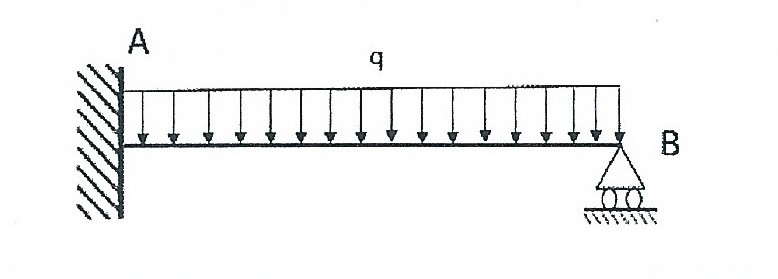
\includegraphics[width=0.7\textwidth]{Enoncedeux}
 \caption{}
 \label{poutre2}
\end{figure}

\end{enumerate}

\subsection{Partie 2}

Dans cette partie on se propose d'étudier la stabilité de la structure représentée à la figure \ref{poutre3}. La poutre est de longueur $L$, encastrée en A, simplement appuyée en B et soumise à une force de compression horizontale $F$ appliquée en B.

\begin{figure}[!ht]
 \centering
 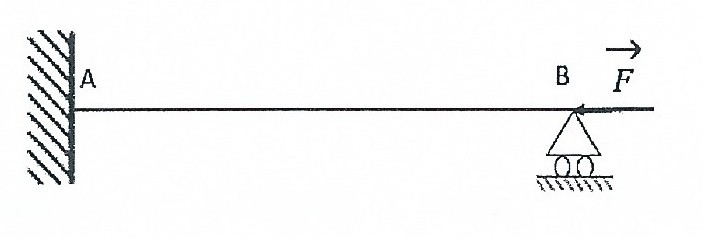
\includegraphics[width=0.7\textwidth]{Enoncedeux2}
 \caption{}
 \label{poutre3}
\end{figure}

\begin{enumerate}
 \item Ecrire les équations régissant le problème de stabilité.
 \item Intégrer l'équation différentielle et calculer les constantes d'intégration.
 \item Calculer le premier mode et la charge critique de flambement que l'on notera $F_c$ (une solution approchée de $\tan(x)=x$ est $x=4.493$).
 \item Donner une approximation de $F_c$ en utilisant la méthode énergétique approchée et la comparer à la valeur exacte.
\end{enumerate}

\begin{solution}

\textbf{Partie I - poutre chargée}

1. Nous allons travailler dans la configuration déformée. En outre, nous supposerons, au début, que $V_B$ nous est donnée. Nous calculons le moment fléchissant au moyen de deux coupes :

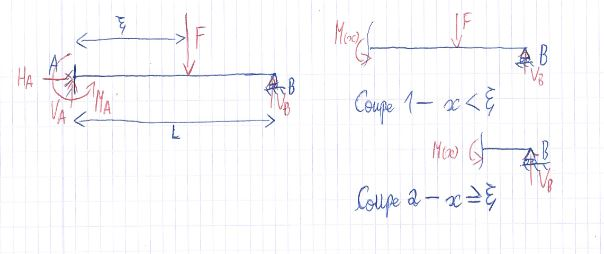
\includegraphics[scale = 0.75]{poutres.jpg}

$$H_A = 0$$
$$V_A = F - V_B,$$ 
$$M(x) = F( \xi - x) - V_B(L - x)$$

L'énergie de déformation $W = \frac{1}{EI}\int _0 ^L M^2 (x) dx$.

 Si $x \leq \xi$ : $M^2(x) = F^2(\xi - x)^2 + V_B^2 (L-x)^2 -2V_B F (\xi - x)(L - x)$

 Si $x \geq \xi$ : $M^2(x) = V_B^2 (L-x)^2$

$$\int _0 ^{\xi} M^2(x) dx = [\frac{x^3}{3}V_B^2 - \frac{x^2 L}{2}V_B^2 + xL^2V_B^2 - 2V_B F(\frac{x^3}{3} - \frac{x^2}{2}(L + \xi) + \xi Lx)]_0^{\xi}$$ 
$$= \xi^3 V_B (\frac{V_B}{3} - \frac{2}{3}V_B +V_B) + \xi^2LV_B (- \frac{V_B}{2} + \frac{F}{2} -2F) + \xi L^2 V_B^2$$

où le terme en $F^2$ n'a pas été calculé car ce terme sera dérivé, exclusivement, par rapport à $V_B$ par la suite...

$$\int _{\xi} ^{L} M^2(x) dx = [V_B^2 (\frac{V_B}{3} - \frac{2}{3}V_B +L^2x)]_{\xi}^L = V_B^2 (\frac{L^3}{3} - \frac{L^3}{2} + L^3 + \frac{\xi ^3}{3} -\frac{\xi ^2}{2}L + \xi L^2)$$

$$\frac{\partial W}{\partial V_B} = \frac{1}{2EI}\frac{\partial}{\partial V_B} (V_B^2 (\xi^3 - \xi ^2 L + 2\xi L^2+\frac{5}{6}L^3) + FV_B(-\frac{3}{2}\xi ^2L)$$

$$= \frac{2V_B}{2EI}(\xi^3-\xi^2 L + 2\xi L^2 +\frac{5}{6}L^3) -\frac{3}{4EI}F\xi^2 L = u(L)$$
Où la dernière égalité a été donnée en vertu du théorème de Castigilano. 

Puisque $u(L) = 0$, on trouve 
$$V_B = \frac{3}{4}\frac{\xi^2 L}{\xi ^3 -\xi^2 L + 2 \xi L^2 + 5/6 L^3} F$$
et on en déduit que 
$$V_A = F - V_B = (1 - \frac{3}{4}\frac{\xi^2 L}{\xi ^3 -\xi^2 L + 2 \xi L^2 + 5/6 L^3}) F $$
$$M_A = F\xi - V_B L = (\xi - \frac{3L}{4}\frac{\xi^2 L}{\xi ^3 -\xi^2 L + 2 \xi L^2 + 5/6 L^3}) F$$

2. Pour représenter les moments, nous avons utilisé (de manière tout à fait arbitraire) la relation de proportionnalité $V_B = \frac{1}{2}F$, et

\begin{align*}
    M(x) & = F(\xi - x) - V_B(L-x) & Q(x) & = -F + V_B & N(x) &= 0 & (\forall x \in [0, \xi])\\
         & = -V_B(L - x)            &      & = V_B      &      &= 0 & (\forall x \in [\xi, L])
\end{align*}

3. Puisque $M(x) = -EI v''(x)$, on trouve les EDO suivantes :

 - (a) Sur $[0, \xi]$ : $v''(x) = -\frac{1}{EI}(F(\xi - x) - V_B(L-x))$. 

Par intégration, 
$$v(x) = x^3 (\frac{F-V_B}{6EI}) + \frac{x^2}{2EI}(F\xi - LV_B) +Ax + B,$$
avec $v(0) = B = 0$ et $v'(0) = A = 0 \Rightarrow v(x) = \frac{F - V_B}{6EI}x^3 + \frac{F\xi - LV_B}{2EI}x^2$

 - (b) Sur $[\xi, L]$, $v''(x) = -\frac{1}{EI}(- V_B(L-x))$.

Par intégration, 
$$v(x) = \frac{1}{EI}(-V_B\frac{x^3}{6} + L\frac{x^2}{2}) + Ax + B,$$

avec les C.L. $v(L) = 0$, et $v(\xi) = v_1(\xi)$, où on appelle $v_1(\xi)$ la valeur trouvée en (a) en ce point (continuité de la poutre !).

4. Par le principe de Saint-Venant, les réactions aux appuis calculés au point 1. sont conservées. L'effort normal reste nul, mais nous avons désormais

\begin{center}

$M(x) = \frac{(L - x)^2}{2} q$  et  $Q(x) = q(2L-x)$

\end{center}

A l'aide ce ce moment, nous avons utilisé la même méthode pour le calcul de la flèche. Nous prenons pour conditions aux limites :

$$v(x) = v(0) = 0 = v'(0)$$

$$v(x) = \frac{-q}{EI}(\frac{x^4}{12} - \frac{L}{3}x^3 + \frac{L^2}{2}x^2) + Ax + B$$

\textbf{Partie II - Flambement}

Précisons d'abord que nous allons travailler dans la configuration déformée $v(x)$ représentée ci-dessous , mais sous hypothèses de perturbations suffisamment petites pour qu'on puisse négliger le déplacement selon x :

\newpage

\begin{center}

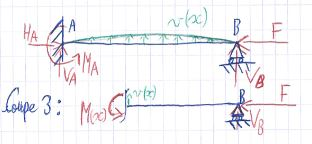
\includegraphics[scale = 1]{Flambement.jpg}

\end{center}

Par l'équilibre des forces et des moments,

\begin{center}
    $H_A = F$, et $V_A = - V_B$
\end{center}

On déduit immédiatement les moments de flexion, et l'EDO pour les déplacement, avec $V_B$ inconnu :

\begin{align*}
     M(x) = Fv(x) - V_B (L - x) &= -EIv''(x)\\
     v''(x) + \frac{F}{EI} v(x) &= - V_B (L - x)
\end{align*}

2. La solution générale est de la forme $v(x) = A\sin(kx) + B\cos(kx) +\frac{V_B}{F}(L-x)$, avec $k = \sqrt{\frac{F}{EI}}$. On impose également $v(0)= v'(0) = 0 = v(L) $. Par les conditions sur v en 0 : 

$$A = \frac{V_B}{Fk}$$
$$B = -\frac{V_B L}{F}$$

3. En L, 
$$v(L) = A \sin(kL) + B\cos(kL) = 0 = \frac{V_B}{kF}\sin(kL) - \frac{V_B L}{F}\cos(kL)$$

$$kL = \frac{\sin(kL)}{\cos(kL)} = tg(kL)$$

Une valeur approchée nous est fournie dans l'énoncé : 

$$kL = 4.493 \Rightarrow k = \frac{4.493}{L}$$ 

Il reste à appliquer la définition de $k$ : $ k = \sqrt{\frac{F}{EI}}$, et nous déduisons que 

$$\sqrt{F_{c}} = \sqrt{EI}\frac{L}{4.493} \Rightarrow F_{c} = EI\frac{L^2}{4.493^2}$$

4. A faire...

\end{solution}

\section{}

\textit{Les calculs doivent être détaillés, les résultats finaux ne seront pas acceptés.}

\medskip
On étudie les vibrations libres d'une structure comprenant deux poutres rigides soutenues par deux rotules fixes et par des ressorts.
La poutre inférieure a une longueur $2L$ et une masse $2m$ et la poutre supérieure, une longueur $L$ et une masse $m$. Les deux poutres forment des angles $\psi$ et $\theta$ par rapport à l'horizontale. Tous les ressorts ont un allongement nul lorsque $\psi=\theta=0$. On suppose les ressorts verticaux.

\begin{figure}[h!]
 \centering
 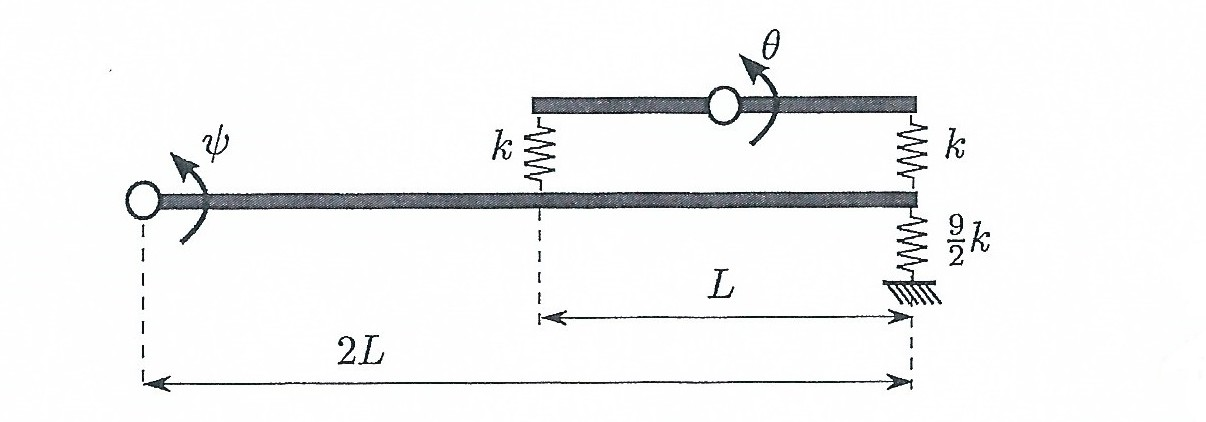
\includegraphics[width=0.7\textwidth]{Enoncetrois}
\end{figure}

On choisit comme coordonnées généralisées: 
\[
 \underset{\sim}{x}=\begin{pmatrix}
L\,\psi \\ L\,\theta
\end{pmatrix}
\]

qui représentent les positions des poutres par rapport aux positions d'équilibre statique.

\begin{enumerate}
 \item Donnez l'expression de l'énergie potentielle de la structure en tenant compte des termes associés à la gravité.
 \item Déterminez la positon d'équilibre en fonction de $\psi$ et $\theta$.
 \item Donnez l'expresion de l'énergie cinétique de la structure.
 \item Calculer les matrices de masse et de raideur en fonction des coordonnées généralisées. On rappelle les équations de Lagrange:
 
    \[ L_{lag}=\mbox{énergie cinétique $-$ énergie potentielle} \]
    \[ \frac{d}{dt}\frac{\partial L_{lag}}{\partial \dot{x}_i}-\frac{\partial L_{lag}}{\partial x_i}=0 \]
 
 avec $x_i$ les composantes des coordonnées généralisées.
 \item On considère dorénavant que la position d'équilibre correspond à $\psi=\theta=0$. Calculer les pulsations propres du système en utilsant les matrices de masse et de raideur suivantes;
 \[
  \mathbf{M}=\frac{m}{12} \begin{pmatrix} 32 & 0 \\ 0 & 1 \end{pmatrix}
  \qquad
  \mathbf{K}=\frac{k}{2} \begin{pmatrix} 46 & -1 \\ -1 & 1 \end{pmatrix}
 \]
 
 \item Les deux poutres sont initialement maintenus inclinées par rapport à l'horizontale de manière telle que $\theta=-2\psi=\theta_0$ et leur vitesse initiale est nulle. La relation $\theta=-2\psi$ reste-t-elle valable lorsqu'on relâche les poutres pour les laisser osciller librement autour de la position d'équilibre? Justifiez précisément votre réponse.
 
\end{enumerate}

\begin{solution}

\begin{enumerate}
 \item L'énergie potentielle due aux ressorts est modélisée par la relation $E_{p,k} = \sum_{i=1}^3 k_i\frac{x_i^2}{2}$, où $x_i$ et $k_i$ sont, respectivement, l'allongement (par rapport à la longueur neutre) et la rigidité de chacun des trois ressorts.

$$\underline{k} = \left(k, k, \frac{9}{2}k\right), \quad \underline{x} = \left( -L \sin(\psi) - \frac{L}{2}\sin(\theta), -2L \sin(\psi) + \frac{L}{2}\sin(\theta), 2L \sin(\psi)\right) $$
    
$$E_{p,k} = \frac{k}{2}\left(\left(L \sin(\psi) + \frac{L}{2}\sin(\theta)\right)^2 + \left(2L \sin(\psi) - \frac{L}{2}\sin(\theta)\right)^2 + \frac{9}{2} 4L^2\sin^2(\psi)\right)$$

$$E_{p, G} = mgh = \frac{2m}{2L}g \int_0^{2L} x \sin(\psi) dx + 0 = 2 mgL \sin(\psi)$$

L'énergie potentielle due à la gravité est nulle pour la barre supérieure puisque cette barre tourne autour de son centre de masse.

$$E_p = E_{p, k} + E_{p, G} = \frac{kL^2}{2}\left(23 \sin^2(\psi) - \sin(\psi)\sin(\theta) + \frac{1}{2} \sin^2(\theta)\right) + 2 mgL \sin(\psi)$$

\item Les conditions pour que le système soit à l'équilibre sont $E_p = \underset{\underline{x}}{min} (E_p)$ et $\underline{\overset{\textbf{.}}{x}} = 0$. Supposons donc une vitesse angulaire nulle dans une configuration telle que :

$$\frac{kL^2}{2}(23 \sin^2(\psi) - \sin(\psi)\sin(\theta) + \frac{1}{2} \sin^2(\theta)) + 2 mgL \sin(\psi) = 0,$$

C'est à dire (simplement !) que $\theta = \psi = 0$.

\item Pour l'énergie cinétique,

$$E_k = \frac{2m}{2L} \frac{1}{2} \int_0^{2L} (x \overset{\textbf{.}}{\psi})^2 dx + \frac{m}{L}\frac{2}{2} \int_0^{\frac{L}{2}} (x \overset{\textbf{.}}{\theta})^2 dx,$$

où la fraction $\frac{m}{L}\frac{2}{2}$ vient du fait que c'est $E = m\frac{v^2}{2}$ et de la symétrie de la poutre ancrée en $\theta$ (on intègre $v^2$ sur les deux tronçons de longueur $\frac{L}{2}$).

$$E_k = \frac{4mL^2}{3}\overset{\textbf{.}}{\psi}^2 + \frac{mL^2}{24}\overset{\textbf{.}}{\theta}^2$$

\item $$L_{lag} = E_k - E_p = \frac{4mL^2}{3}\overset{\textbf{.}}{\psi}^2 + \frac{mL^2}{24}\overset{\textbf{.}}{\theta}^2 - \frac{kL^2}{2}\left(23 \sin^2(\psi) - \sin(\psi)\sin(\theta) + \frac{1}{2} \sin^2(\theta)\right) - 2 mgL \sin(\psi)$$

Puisque nous sommes en petits déplacements, nous allons utiliser l'hypothèse suivante, sur les sinusoïdes : $\sin(\psi) = \psi$, $\sin(\theta) = \theta$ et $\cos(\psi) = \cos(\theta) = 1$. 

$$L_{lag} = E_k - E_p = \frac{4mL^2}{3}\dot{\psi}^2 + \frac{mL^2}{24}\dot{\theta}^2 - \frac{kL^2}{2}\left(23 \psi^2 - \psi\theta + \frac{1}{2} \theta^2\right) - 2 mgL \psi$$

On rappelle que $\underline{x} = (L\psi, L\theta)$, et dès lors :
    
$$\frac{\partial}{\partial t}\frac{\partial L_{lag}}{\partial \underline{\overset{\textbf{.}}{\psi}}} = \frac{\partial L_{lag}}{\partial \underline{\psi}}$$

$$\frac{\partial}{\partial t}\frac{\partial L_{lag}}{\partial \underline{\overset{\textbf{.}}{\theta}}} = \frac{\partial L_{lag}}{\partial \underline{\theta}}$$

Nos équations se résument à 
$$
\left\{
    \begin{array}{rcl}
         \frac{8}{3}m \ddot{\psi} + \frac{k}{2}(46 \psi - \theta) & = & 2 \frac{mg}{L}\\
         \frac{1}{12} m\ddot{\theta} + \frac{k}{2} (- \psi + \theta) & = & 0
    \end{array}
\right.
$$

\[ 
    M = \frac{m}{12} \begin{pmatrix} 32 & 0 \\ 0 & 1 \end{pmatrix}
    , \qquad
    K = \frac{k}{2} \begin{pmatrix} 46 & -1 \\ -1 & 1 \end{pmatrix}
\] 


\item $\omega_i^2 = \lambda_i$, avec $\lambda_i$ tq 

$$ 
    \det (K - M\lambda_i) = 0 =  \frac{1}{2} 
    \left| \begin{array}{cc}
        46k - \frac{32}{6}m\lambda_i & - k \\
        -k & k - \frac{1}{6}m\lambda_i 
    \end{array} \right|  
$$

$$ \frac{32}{36} m^2 \lambda_i^2 - \frac{32 + 46}{6} mk\lambda_i + 45 k^2 = 0$$

$$\sqrt{\Delta} = \sqrt{169 - 4*5*8} = \sqrt{9} = 3 \Rightarrow \lambda_i = \frac{13mk \pm 3mk}{\frac{16}{9}m^2}$$

\begin{align*}
    \lambda_1 = 9 \frac{k}{m} &, \omega_1 = 3\sqrt{\frac{k}{m}} & \lambda_2 = \frac{45k}{8m} &, \omega_2 = \frac{3}{2}\sqrt{\frac{5k}{2m}}
\end{align*}

Rappelons que ces valeurs de $\lambda$ sont telles que la matrice $(K - M\lambda)$ soit de rang $2 -1 = 1$, c'est à dire, en ce qui nous concerne, telles que nous pouvons définir deux directions principales $\underline{\omega_i}$, chacune associée à l'unique vecteur (ligne de $K - M\lambda_i$) propre de $\lambda_i$. On a :

$$
    (i = 1)  
    \left( \begin{array}{cc}
        46k - \frac{32}{6}\frac{45}{8}k & - k \\
        -k & k - \frac{1}{6}\frac{45}{8}k 
    \end{array} \right) = 0 
    \Rightarrow \underline{\omega_1} = (2, -1)
$$

$$
    (i = 2) 
    \left( \begin{array}{cc}
        46k - \frac{32}{6}m\lambda_i & - k \\
        -k & k - \frac{1}{6}m\lambda_i 
        \end{array} \right)  
    = 0 \Rightarrow \underline{\omega_2} = (16, 1)
$$

\item La solution qui montre l'évolution temporelle de $ \underset{\sim}{x} $ est une combinaison linéaire des deux directions principales. Puisque $\theta = -2 \psi$ correspond au vecteur propre $\underline{\omega_1}$, cette condition initiale fixe à 0 la constante qui multiplie le second vecteur propre. Les barres vont donc évoluer en vérifiant toujours la relation $\theta = -2 \psi$, c'est-à-dire en restant parallèles.

\end{enumerate}

\end{solution}

\end{document}
